\centering
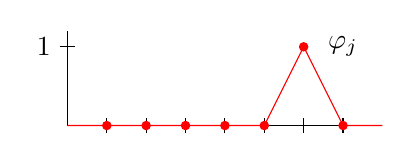
\begin{tikzpicture}[scale=1]

% Achsen
\draw (0,0) -- ++(0,1.2);
\draw (0,0) -- ++(4,0);

% Funktion
\draw[red] (0,0) -- ++(2.5,0) -- ++(0.5,1) -- ++(0.5,-1) -- ++(0.5,0);
	
% Anstrich Y-Achse 
\draw (-0.1,1) -- ++(0.2,0);
	
% Anstriche X-Achse
\draw (0.5,-0.1) -- ++(0,0.2);
\draw (1  ,-0.1) -- ++(0,0.2);
\draw (1.5,-0.1) -- ++(0,0.2);
\draw (2  ,-0.1) -- ++(0,0.2);
\draw (2.5,-0.1) -- ++(0,0.2);
\draw (3  ,-0.1) -- ++(0,0.2);
\draw (3.5,-0.1) -- ++(0,0.2);
	
	
\filldraw[red] (0.5,0) circle (1.5pt);
\filldraw[red] (1  ,0) circle (1.5pt);
\filldraw[red] (1.5,0) circle (1.5pt);
\filldraw[red] (2  ,0) circle (1.5pt);
\filldraw[red] (2.5,0) circle (1.5pt);
\filldraw[red] (3  ,1) circle (1.5pt);
\filldraw[red] (3.5,0) circle (1.5pt);
	
	
\node at (-0.3,1) {1};
\node at (3.5,1) {$\varphi_j$};
\end{tikzpicture}
